\documentclass{beamer}
\usetheme{Antibes}
\usecolortheme{dove}
%\usepackage{FiraSans}

\setbeamertemplate{navigation symbols}{}
\setbeamertemplate{itemize items}[default]
\setbeamertemplate{enumerate items}[default]


\usepackage[spanish]{babel}

\title{Atmósfera de Saturno}
\author{Benjamín Ortiz Edwards}

\begin{document}

\frame{\titlepage}

\section{Saturno}

\begin{frame}


\vspace{-2cm}
\begin{figure}
    \centering
    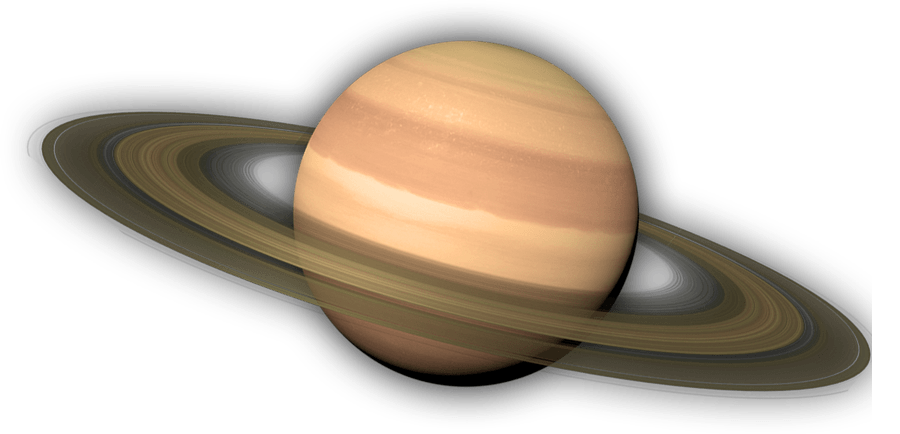
\includegraphics[width=0.6\linewidth]{saturn}
\end{figure}
\begin{enumerate}
    \item Saturno es el sexto planeta más cercano al sol
    \item Su extructura es mayoritariamente gaseosa y líquida, pero con un núcleo sólido
    \item Su apariencia es de colores amarillos y paste, aunque azulado hacia los polos
\end{enumerate}
\end{frame}


\section{Composición y estructura}
\begin{frame}{Composición}
    \begin{itemize}
        \item 75\% de Hidrógeno y 25\% de Helio.
        \item Trazas de	metano, vapor de agua, amoniaco, monoxido de carbono, hidrocarburos, entre otros.	
    \end{itemize}
\end{frame}

\begin{frame}{Estructura}
    \begin{itemize}
        \item La primera capa es de hidrógeno líquido, luego sigue la atmósfera de H y He, con un espesor de 30000 Km.
        \item Posee bandas ecuatoriales, similares a las de Júpiter
            \vspace{\baselineskip}
    \end{itemize}
    \centering
    \begin{tabular}{|l|l|l|l}
        Nubes/Capa & Temperatura & Presión & Composición\\ \hline
        Nubes altas & $\sim$ (100 - 160) K & $\sim$ (0.5 - 2) bar & Amoniaco\\
        Nubes bajas$^1$ & $\sim$ (185 - 279) K & $\sim$ (2.5 - 9) bar & Agua-hielo \\ 
        Nuebs bajas$^2$ & $\sim$ (190 - 235) K & $\sim$ (3 - 6) bar &  NH$_4$SH \\
        Capa inferior & $\sim$ (270 - 330) K & $\sim$ (10 - 20) bar & Solución acuosa
    \end{tabular}`
\end{frame}

\section{Características}
\begin{frame}{Características}


    \begin{itemize}
        \item Se han detectado vientos en la cima de las nubes que alcanzan velocidades de 1800 Km/h (en el ecuador)
        \item En el polo sur hay tiene un vórtice.

            \vspace{1cm}
    \begin{figure}
        \centering
        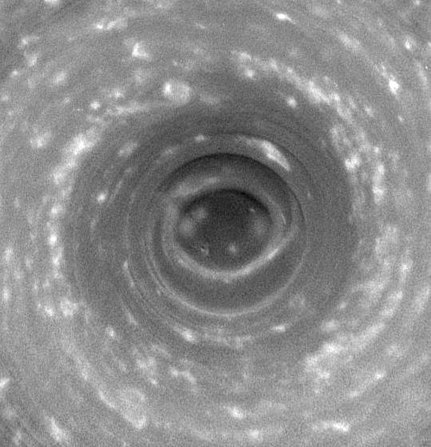
\includegraphics[width=0.3\linewidth]{polar_vortex}
    \end{figure}

    \end{itemize}

\end{frame}


\section{Fenómenos interesantes}
\begin{frame}
    \begin{itemize}
        \item Gran Mancha Blanca.
            \begin{figure}
                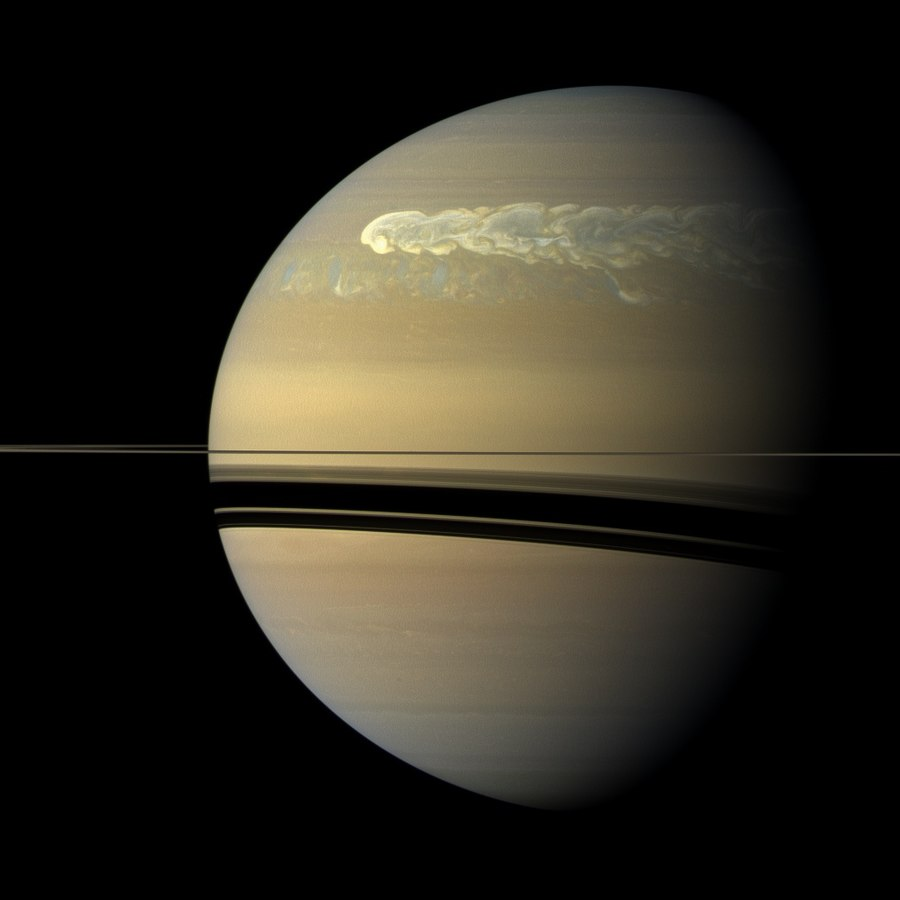
\includegraphics[width=0.35\linewidth]{gws}
            \end{figure}
        \item Nubes hexagonales.
            \begin{figure}
                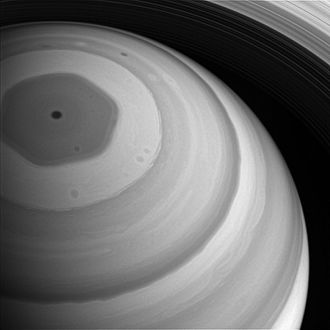
\includegraphics[width=0.35\linewidth]{hexagon}
            \end{figure}

    \end{itemize}
\end{frame}

\section{Algunas Características}


\section{Referencias}

\begin{frame}{Referencias}
\begin{itemize}
    \item https://www.esa.int/Science\_Exploration/Space\_Science/Cassini-Huygens/Saturn\_s\_atmosphere
    \item ``Saturn from Cassini-Huygens'', Dougherty, Michele K. ; Esposito, Larry W. ; Krimigis, Stamatios M.
        Abstract

    \item ``A hexagonal feature around Saturn's north pole'', D.A.Godfrey

\end{itemize}
\end{frame}




\end{document}
